\section{Block Diagram}

Figure~\ref{fig:blockDiagram} shows a revised system block diagram. It contains the model numbers of all the components, the types of connections required to the microcontroller unit (MCU) and the amount of lines needed for each connection. An explanation of the changes made follows. The changes stated in this section, are not only reflected in the block diagram but also in the system schematic shown in the following section.

\begin{figure}[H]
\centering
	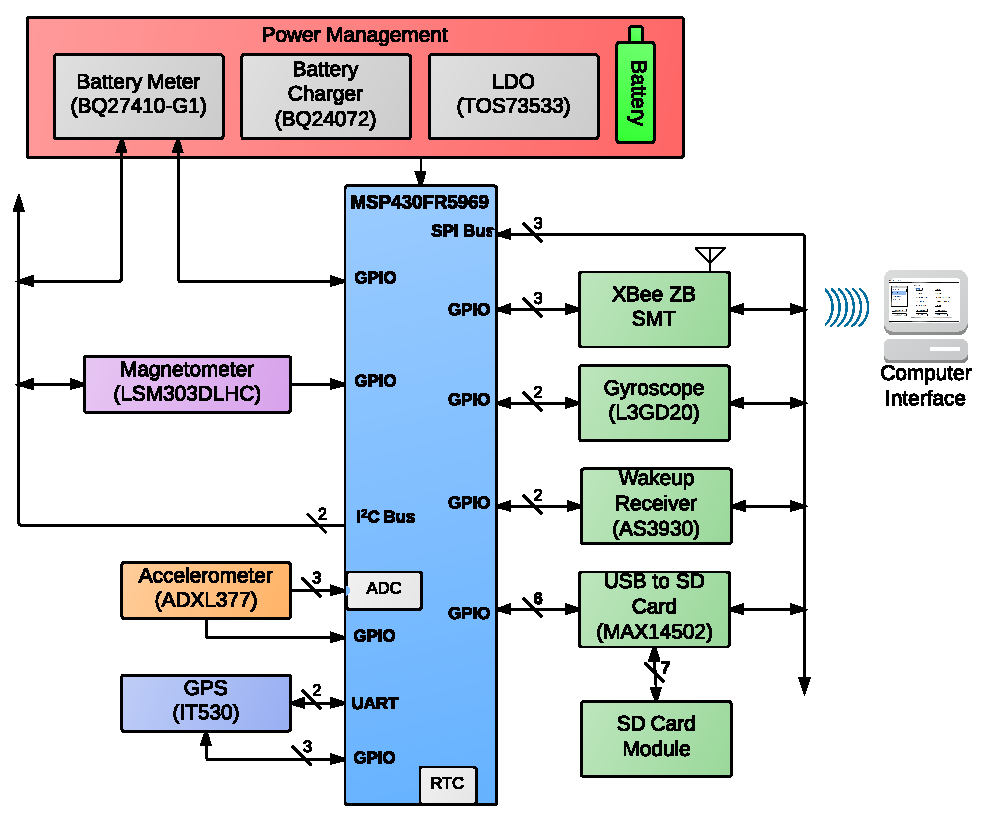
\includegraphics[width=\textwidth]{img/blockDiagram}
	\caption{System Block Diagram \label{fig:blockDiagram}}
\end{figure}

\subsection{Battery Charger and Battery Meter}

In the thermal analysis previously performed, it was found that the power loss in the LDO conversion was too high, because the input, which came from the battery charger, was 5V, while the output was 3.3V to comply with the specifications for our components.  To avoid such power loss, the battery charger was changed to a BQ24072 which has a regulated output voltage equal to the battery voltage plus 225 mV.  Since the battery voltage is 3.7V, the power loss when converting to 3.3V is significantly reduced.  This not only helps to extend the effective battery life but also to lower the junction temperature significantly.

We had previously used an application note \cite{batMeterAppNote} from Texas Instruments that presented the design for a battery charging/meter circuit.  However, this design coupled together the BQ24075 charger with the BQ27505 fuel gauge, which is why this fuel gauge was chosen.  However, the presented circuit was incompatible with the newly chosen BQ24072 charger, so the fuel gauge was changed as well to the BQ27410.


\subsection{Xbee and GPS}

Xbees have two modes of operation: Transparent (AT) mode and API mode. API mode requires larger packets to send information, in addition to encryption and decryption functions.  This translates to the need of more RAM and program memory, more time to send data and higher power consumption.  AT mode, on the other hand, is a very simple and fast mode to communicate between Xbees. Since this system is battery driven, it needs to have a very low power consumption.  The system also needs to transfer data between the base station and the sphere as quickly as possible because the available time to send or receive data is very short in some cases.  Also, because a lot of components are being used, memory is a valuable and limited resource in this system. All these facts make AT mode more feasible for the application. Previously, it was stated that the communication between the Xbee and the MCU was going to be made via SPI. Because SPI mode requires the use of API mode while AT mode is only available when communicating with the Xbee via UART, the communication with this component was changed from SPI to UART.

With this change, another problem arose - the chosen MCU did not have an additional UART port available because it was being used for the GPS module. Two ways to make the Xbee UART communication possible were considered.  The first method considered was the addition of a multiplexer to the UART line to allow the two components to communicate with the MCU via the same UART lines.  This implies the addition of another hardware component to the system.  Since the system has space limitations, this option was not very feasible.  Also, adding extra components implies a higher power consumption.  The second method considered was to implement UART via software.  Implementing a software UART is very simple and does not require much program memory. Since the Xbee is going to be used more than the GPS, it is best to connect the Xbee to the hardware UART for efficiency purposes.  This will help save CPU cycles and thus save more power.  The GPS module will then be connected to the newly software UART ports.

